Equilíbrio ácido-base.

O gráifco abaixo representa o progresso da titulação do aminoácido com equivalentes de \chemfig{NaOH}.

\begin{center}
	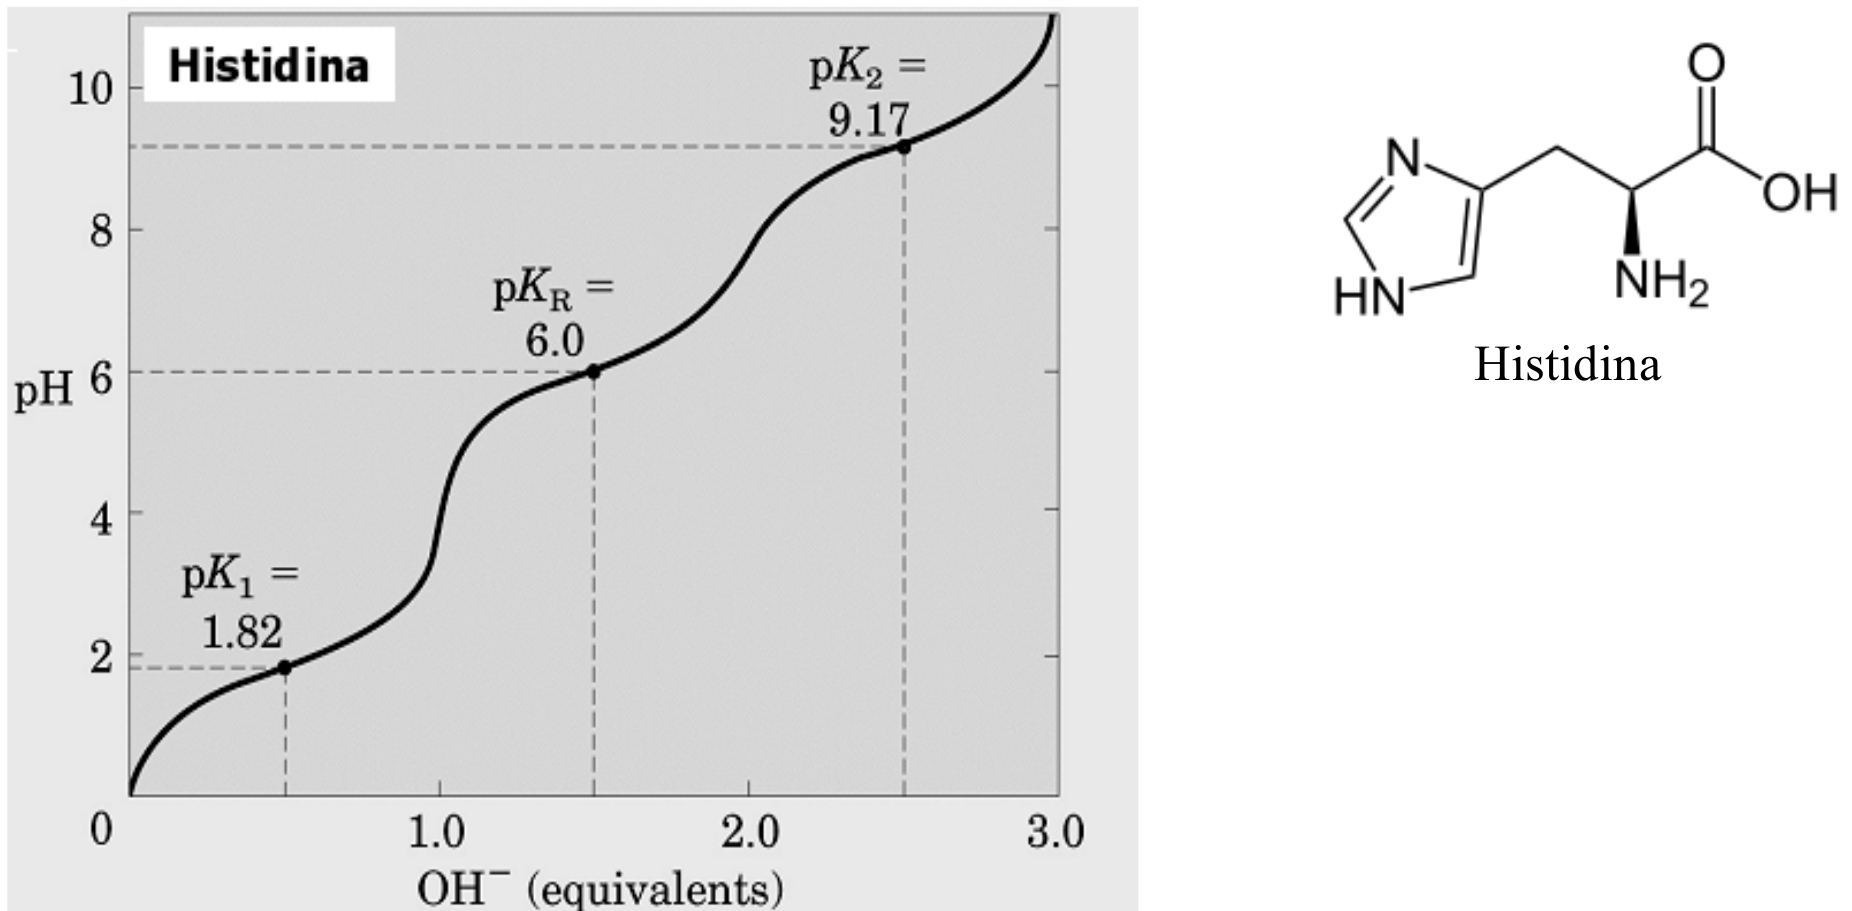
\includegraphics[width = 0.8\textwidth]{figure.png}
\end{center}

\begin{enumerate}[label = (\alph*)]
	\item Apresente todos os equilíbrios de ionização relevantes para a histidina, indicando para cada um deles o pK relacionado.
		Indique, também, as zonas de maior capacidade tamponante para este aminoácido.

	\item Para reproduzir o meio intracelular em laboratórios de bioquímica, tampões de fosfato são utilizados.
		Considerando que o pH intracelular seja igual a 7,4 e que a solução utilizada para o preparo do tampão tenha $[\chemfig{PO_4^{3-}}] = 0,01$ mol$\cdot$L$^{-1}$, calcule o volume de \chemfig{HCl} $6,00$ mol$\cdot$L$^{-1}$ que deve ser adicionado a $500$ mL dessa solução, para obtenção da solução desejada.
\end{enumerate}
